\documentclass{scrreprt}
\usepackage{selinput}
\usepackage[ngerman,english]{babel} % Standard: English
\usepackage{graphicx}
\usepackage{varioref}

\usepackage{color}
\definecolor{lightgray}{gray}{0.95}




%%%%%%%%%%%%%%%%%%%%%%%%%%%%%%
% For including Java-sources %
%%%%%%%%%%%%%%%%%%%%%%%%%%%%%%

\usepackage{listings}
\lstset{
   language=Java,
   backgroundcolor=\color{lightgray},
   extendedchars=true,
   basicstyle=\footnotesize\ttfamily,
   showstringspaces=false,
   showspaces=false,
   frame=leftline,
   numbers=left,
   numberstyle=\tiny, % or e.g. \footnotesize
   numbersep=9pt,
   tabsize=2,
   breaklines=true,
   showtabs=false,
   captionpos=b,
}




%%%%%%%%%%%%%%%%%%%%%%%%%%%%%%
% Definitions for signatures %
%%%%%%%%%%%%%%%%%%%%%%%%%%%%%%
\newcommand*{\TwoSignatures}[2]{%
\vspace{1.2cm}
\noindent\begin{tabular}{ll}%
\makebox[6.8cm]{\hrulefill} & \makebox[6.8cm]{\hrulefill}\\
#1 & #2
\end{tabular}

}
\newcommand*{\ThreeSignatures}[3]{%
\vspace{1.2cm}
\noindent\begin{tabular}{lll}%
\makebox[4.4cm]{\hrulefill} & \makebox[4.4cm]{\hrulefill} & \makebox[4.4cm]{\hrulefill}\\
#1 & #2 & #3
\end{tabular}
}




%%%%%%%%%%%%%%%%%%%%%%%%%%%%%%
% For cites and bibliography %
%%%%%%%%%%%%%%%%%%%%%%%%%%%%%%
\usepackage[babel,german=guillemets]{csquotes}
\usepackage[backend=biber]{biblatex}
\addbibresource{bibliography.bib}

\usepackage{graphicx} %package to manage images
\graphicspath{ {includes} }

\begin{document}
\titlehead{\centering
\includegraphics[height=2cm]{includes/logo}}
\subject{OOP-Project SS17---Biemann}
\title{Project Delivery}
\subtitle{Group A (Project Title)}
\author{Doe, John\\Mustermann, Martin\\Luke, Lucky}%Use format lastname, surname in separated lines for each participant
\date{\today}
\maketitle


% First of all you have to print and sign the German Affirmation
% Please do not mind about the German Umlauts, because we did not load the correct encoding for German which isn't necessary for an english project.
\selectlanguage{ngerman} % Switch to German for hyphenation and German date format.
\chapter*{Eidesstattliche Erkl\"arung}
Ich erkl\"are hiermit an Eides statt, dass ich die vorliegende Arbeit selbst\"andig und ohne unerlaubte fremde Hilfe angefertigt, andere als die angegebenen Quellen und Hilfsmittel nicht benutzt habe. Die aus fremden Quellen direkt oder indirekt \"ubernommenen Stellen sind als solche kenntlich gemacht.
Die Arbeit wurde bisher in gleicher oder \"ahnlicher Form keinem anderen Pr\"ufungsamt vorgelegt und auch nicht ver\"offentlicht.

\vspace{3mm}\today
\selectlanguage{english} % Back to English

% Do not forget your signatures
%\TwoSignatures{John Doe}{Martin Mustermann} % For four signatures use it twice
\ThreeSignatures{Martin Mustermann}{John Doe}{Lucky Luke}


%%%%%%%%%% Let's start %%%%%%%%%%
\tableofcontents


% The following is an idea for a structure you can use. Feel free to adapt this to your needs.
% Remark: Sectioning makes only sense if you have enough content/text. Avoid sections with less than a few lines of text.
\chapter{Idea and Motivation}
In this chapter you should write about the initial idea and your applications intention at the start of the project.
For a repetition you can add your mockups e.g.\ as seen in figure~\vref{mockup}.
% In the final document you should have quite more text than in each weekly report. And you should have more than one figure which should float in the document to an adequate position. For this use the figure-environment:
\begin{figure}
    \centering
    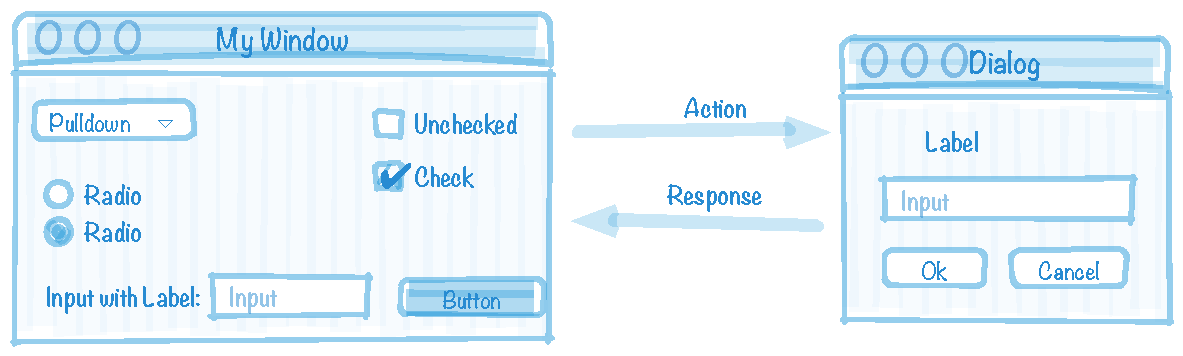
\includegraphics[width=14.6cm]{includes/mockup}
    \caption{First mockup of the prototype}
    \label{mockup}
\end{figure}


\chapter{Realization}
Here you write down what you have done.
Split your document-structure into your proceeding (weekly reports) and each member.
Add also failures and not only successes.
Do not forget any ressources you have used and cite them like in~\cite{example:article} or~\cite{example:url}.
Use UML-diagrams (see fig.~\vref{uml}) of important parts of your object-oriented design or other illustrations as in figure~\vref{erd} if needed.
\begin{figure}
    \centering
    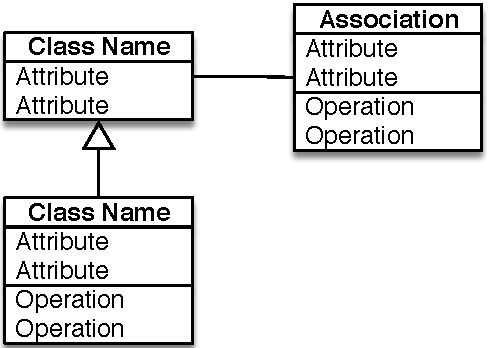
\includegraphics[scale=0.8]{includes/uml}
    \caption{UML-diagram used for the database-connection}
    \label{uml}
\end{figure}
\begin{figure}
    \centering
    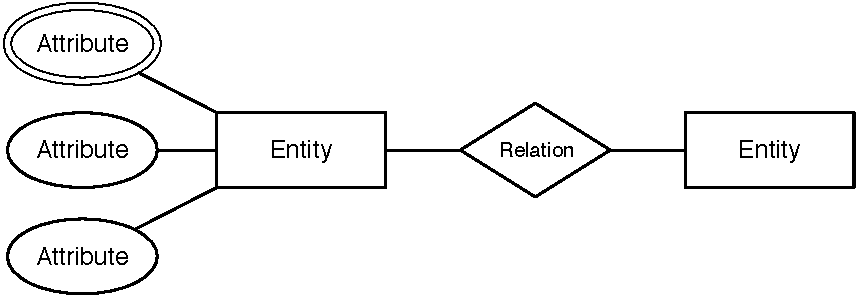
\includegraphics{includes/erd}
    \caption{ER-diagram of the database}
    \label{erd}
\end{figure}%
Maybe drop some lines of the essential parts of your source-code as shown in the listing~\vref{hello}.
\begin{lstlisting}[caption={Hello World example in Java}, label={hello}]
public class HelloWorld {
	public static void main(String[] args) {
		System.out.println("Hello World");
	}
}
\end{lstlisting}

Indeed this section is important for the examination. So outline your work and knowledge so that we can talk about in the oral-exam.


\chapter{Final Version}
Describe your final project result.


\section{Installation}
If you need some special knowledgde about the installation, mention this here.


\section{Quick Start Manual}
What should the user know to get a quick start into your application?


\chapter{Conclusion}
Some final words


\printbibliography

\end{document}
